%!TEX root = ../thesis.tex

\thispagestyle{myheadings}

\graphicspath{{Body/Figures/RatioAnalysis/}{Body/Figures/RatioAnalysis/MethodOverview/}}

\chapter{\texorpdfstring{\wa}{wa} Measurement}
\label{chapter:SpinPrecessionMeasurement}


The measurement of \wa is determined by counting the number of detected positrons in the calorimeters above some energy threshold, as described in \secref{section:WaIntro}. Doing so results in a histogram of counts which is modulated by \wa, \figref{fig:gm2wiggle}. Fitting for the frequency allows \wa to be extracted. The \wa measurement therefore consists of the steps needed to construct the histogram of counts, and the fitting of said histogram.


\section{Reconstruction}
\label{sec:ReconWest}


The calorimeters measure hit times and energies of impacting particles, where these hit times and energies are determined from SiPM current signals and a reconstruction procedure. The reconstruction procedure consists of the steps need to take the raw signals and produce correct measurements of the positron energies and times. In E989 there are two separate reconstruction algorithms, \texttt{ReconWest} and \texttt{ReconEast}. Using separate reconstruction methods gives confidence in any final results be removing any single points of failure. The reconstruction method used in this analysis is \texttt{ReconWest}. A summary of its details will be presented here. A more thorough description is detailed by A. Fienberg \cite{AFThesis}.


The raw data are digitized waveforms, which are voltage versus time signals output from each SiPM. Due to the incredible amount of data coming in with the high muon fill rate, only those traces which exceed some threshold are saved to disk. An online processing system checks the traces against this preconfigured threshold by passing all of the data through a GPU farm \cite{Gohn:2016shi}. If any trace is found above threshold, then the data is saved from every SiPM in every calorimeter, for a time range around the over-threshold pulse. This time range is called a time island, similar to in the tracking reconstruction, and typically has a width of $\SI{40}{ns}$ \cite{AFThesis}. These traces are corrected for undesired digitzer effects.


The trace pulses are then fit with templates in order to extract the pulse area and peak times. Each SiPM has its own templates, one for positrons and one for laser pulses. These templates are extracted from data, where each template is determined by collecting many traces from a SiPM, normalizing by pulse area, aligning in time, and averaging them. These templates were checked against many systematic effects in order to make sure that the constructed templates did not bias the energy or time measurements, such as hit angle, energy (pulse size), position, and rate, and aging \cite{Kaspar:2016ofv,AFThesis}. Each trace is fit using a \chisq minimization algorithm with the corresponding SiPM templates in order to determine the time and energy of the hit. In order to fit for multiple pulses in a single trace or time island, the fitting procedure first fits with a single template, and then checks the residuals for any remaining peaks. If peaks exist above some threshold, then the fitting is repeated until all pulses have been fit. The time measurement performance in the pulse finding was found to be unaffected by the number of pulses in a trace, and there is 100\% pileup separation at \ns{5} \cite{AFThesis}. 


\textbf{probably a picture of a pulse and template here - single, potentiall a multi pulse fit as well, template fit per crystal..}


Once the pulses have been fit with the template, the pulse areas need to be converted to real energy units using an energy calibration procedure. A couple of different techniques exist that can be used, including a method that counts photo-statistics seen in the SiPMs. The default method used is a comparison of lost muon energy signatures in the calorimeters. As described in \refref{lostmuons}, muons lost from the storage ring can spiral inward and hit consecutive calorimeters with a specific time separation between calorimeter hits. These lost muons are minimum-ionizing particles, and thus leave a very distinct energy signature in the crystals. Selecting on the time signature allows hits corresponding to lost muons to be isolated, and different channels can be equalized based on the energy signatures. \textbf{Is it a little awkward to talk about lost muons here when I haven't talked about them at all yet?} Finally, determining the energy calibration for positron hits as compared to lost muon hits needs to be done. Again there are a couple of different techniques, including a comparison of endpoint energies for high energy positrons which tail off at the magic momentum of $\SI{3.094}{\GeV}$ and comparing to simulation. The default technique is to calibrate the energies such that the optimal energy threshold for the \wa analyis is $\SI{1.7}{\GeV}$ \cite{AFThesis}. Ultimately the energy calibration doesn't matter too much because it is not the energy units that we really care about. What we really care about is the number of positrons above some energy threshold, where that threshold can be optimized emperically. In fact, besides the use of general physics intuition, the entire \wa analysis could be done without even considering the energy of the incident positrons, and only considering the amplitude of the SiPM pulses. \textbf{Haven't talked about the optimal threshold yet} After the energy calibration is completed the energies of the pulses are modified according to the laser systems measurement of the gain. Systematic effects from this are studied in \secref{sub:gain}. \textbf{Maybe I should be showing gain curves here and talking about it a bit more?}


Each pulse fit now has an energy and a time associated with it. In order to measure \wa to high precision, the time reconstruction of the pulse is the most important part. The fitted pulse times for each pulse need to be aligned both on a fill-by-fill basis relative to the injection time of the beam, corrected for any channel differences due to differing pulse shapes or fiber lengths, and corrected for any calorimeter differences due to the use of different laser system components. The former is corrected for using the T0 detector as described in \secref{sec:T0}. The latter are corrected by aligning calorimeter channels in time using signals from islands with large simultaneous pulses in neighboring crystals, and aligning calorimeters using lost muon coincident events as described before.


The last part of the calorimeter reconstruction is the clustering. Clustering is the stage which takes the individual template fit results from separate crystals, and turns them into the times, energies, and positions of decay positrons impacts. For a time island with a single positron impact, the procedure is pretty straightforward. The energy for the positron hit cluster is the sum of each individual crystal energy hits. The time for the cluster is taken as the time of the maximum energy hit in the island. This works because most of the positrons energy is localized to a single crystal, and is within $\SI{100}{ps}$ of an energy-weighted calculation of the time. The position of the cluster is determined with a logarithmic weighting function, which for a $\SI{2}{\GeV}$ positron in the E989 calorimeters has a resolution of $\SI{2}{mm}$ \cite{AFThesis}. For a time island with multiple positron impacts, the individual crystal hits are separated in time, where the time partitioning separates hits that are $\SI{2.5}{ns}$ apart, and the clustering proceeds as before. For hits which are within this time window, a pileup event has occurred. If the pileup event happens within the same crystal, then the multiple hits are measured as a single hit, and this needs to be corrected for using a pileup subtraction technique, as described in \secref{sub:pileupsubtraction}. For hits that occur in separate crystals, the pileup can be resolved using the spatial separation of the calorimeters. This is an ongoing area of work, and one technique is described in \refref{AFThesis}. For this analysis the spatial separation was turned off, which simplifies the analysis somewhat. This increases the amount of pileup seen in the data, which again is handled by the pileup subtraction technique. For the precision of the Run 1 analysis result, this was found to be acceptable. For the final goal of $\SI{140}{ppb}$ more work will need to be done on this.





-quick summary of reconstruction process







\section{Histogramming}
\label{sec:Histogramming}


Once the reconstruction has processed all the hits into clusters, the time spectra histograms need to be made.



-artificial deadtime
-time randomization

\subsection{Pileup subtraction}
\label{sub:pileupsubtraction}


\section{Lost muons}
\label{sec:lostmuons}


\refref{lostmuons}


\section{Fitting}
\label{sec:Fitting}


-detail the ratio method - might need to pull stuff out from my appendix


    \begin{figure}[]
    \centering
        \begin{subfigure}[t]{0.45\textwidth}
            \centering
            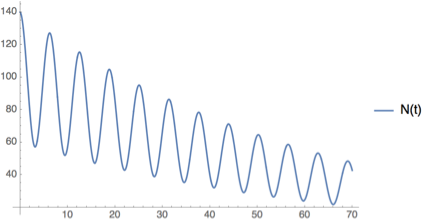
\includegraphics[width=\textwidth]{FiveParamFunc}
            \caption{}
        \end{subfigure}%

        \vspace{2mm}
        \begin{subfigure}[t]{0.45\textwidth}
            \centering
            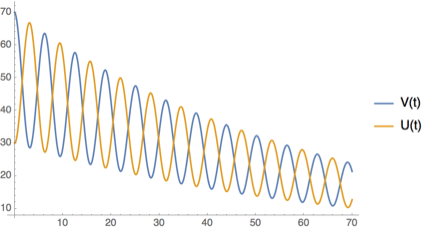
\includegraphics[width=\textwidth]{UVFuncs}
            \caption{}
        \end{subfigure}
        \begin{subfigure}[t]{0.45\textwidth}
            \centering
            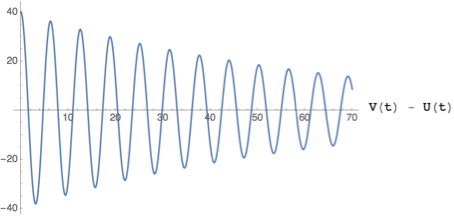
\includegraphics[width=\textwidth]{RatioNumFunc}
            \caption{}
        \end{subfigure}%
        \vspace{2mm}
        \begin{subfigure}[t]{0.45\textwidth}
            \centering
            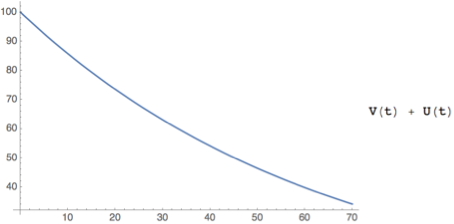
\includegraphics[width=\textwidth]{RatioDenomFunc}
            \caption{}
        \end{subfigure}
        \begin{subfigure}[t]{0.45\textwidth}
            \centering
            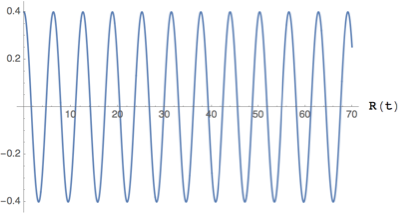
\includegraphics[width=\textwidth]{RatioFunc}
            \caption{}
        \end{subfigure}% 
    \caption[]{}
    \label{}
    \end{figure}






\section{Systematic errors}
\label{sec:Systematic Errors}



\subsection{Gain}
\label{sub:gain}



\cleardoublepage
